\documentclass[xcolor=table]{article}
\usepackage{DejaVuSansMono}
\usepackage{ragged2e}
\usepackage{csquotes}
\usepackage{pstricks}
\usepackage{pst-text}
\usepackage{pst-node}
\usepackage{pst-eps}
\usepackage{savesym}
\savesymbol{checkmark}
\usepackage{dingbat}
\usepackage{anyfontsize}
\usepackage{pifont}
\usepackage{wasysym}
\usepackage{graphicx}
\begin{document}
\psset{unit=1.5in}
\fontfamily{DejaVuSansMono-TLF}\fontsize{50}{50}\selectfont%
\TeXtoEPS
\begin{pspicture}(0,0)(2.5,6.5)
%\rput[bl](0,0){\psgrid(0,0)(3,6.5)}
\rput[bl](0.5,0.5){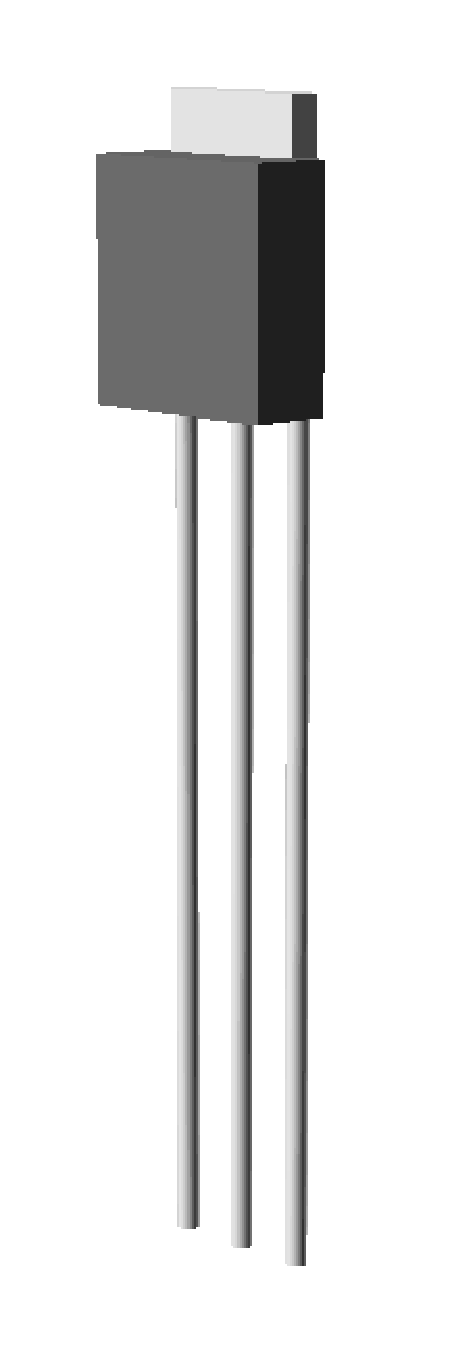
\includegraphics{mosfet.eps}}
	\rput[bl](0.98,0.65){\textcolor{blue}{G}}
	\rput[bl](1.38,0.55){\textcolor{red}{D}}
	\rput[bl](1.75,0.48){\textcolor{black}{S}}
\end{pspicture}
\endTeXtoEPS
\end{document}
